\documentclass{beamer}
%Information
\title{Combination 1: Counting Principle}
\titlegraphic{\hfill
\includegraphics[height=1cm]{orange.png}}
\institute{Youth STEM Academy}
\author{Erzhuo Wang}
\date{\today}
%Theme
\usetheme[block=fill, sectionpage=none]{metropolis}
\useoutertheme{infolines}
\useinnertheme{metropolis}
\setbeamertemplate{blocks}[rounded][shadow=false]
\setbeamertemplate{items}[ball]
\setbeamertemplate{sections/subsections in toc}[ball]
\setbeamertemplate{headline}{}
\logo{YSA}
\usecolortheme{custom}
%\usetheme{Madrid}
%\usetheme{Heverlee}

%Setting
\usepackage[UTF8,noindent]{ctexcap}
\ctexset{today=old}
\theoremstyle{definition}
\newtheorem{defn}{Definition}[section]
\newtheorem{coro}[defn]{Corollary}
\newtheorem{theo}[defn]{Theorem}
\newtheorem{exer}[defn]{Exercise}
\newtheorem{rema}[defn]{Remark}
\newtheorem{lem}[defn]{Lemma}
\newtheorem{prop}[defn]{Proposition}
\newtheorem{nota}[defn]{Notation}
\newtheorem{exam}[defn]{Example}
\newtheorem{ques}[defn]{Question}

\newenvironment{prooff}{{\noindent\it\textcolor{cyan!40!black}{Proof}:}\,}{\par}
\newenvironment{proofff}{{\noindent\it\textcolor{cyan!40!black}{Proof of the lemma}:}\,}{\qed \par}
\newcommand{\bbrace}[1]{\left\{ #1 \right\} }
\newcommand{\bb}[1]{\mathbb{#1}}
\newcommand{\p}{^{\prime}}
\renewcommand{\mod}[1]{(\text{mod}\,#1)}
\newcommand{\blue}[1]{\textcolor{blue}{#1}}
\newcommand{\spec}[1]{\text{Spec}({#1})}
\newcommand{\rarr}[1]{\xrightarrow{#1}}
\newcommand{\larr}[1]{\xleftarrow{#1}}
\newcommand{\emptyy}{\underline{\quad}}
\newenvironment{enu}{\begin{enumerate}[(1)]}{\end{enumerate}}
%ctrl+点击文本返回代码  选中代码 ctrl+alt+j 为代码查找文本

\begin{document}
\begin{frame}
    \titlepage
\end{frame}
% \section{Counting Principle}
% \begin{frame}{Fundamental Counting Principle}
%     \begin{theo}[addition rule]
%         If there are $m$ ways to complete a first task and $n$ ways to complete a second task, then the number of ways to complete
%         one of the two tasks is $m+n$.
%     \end{theo}
%     \begin{exam}
%         If one bowl contains $5$ apples and a second bowl contains $8$ oranges, then there are $5+8$ ways to choose one piece of fruit.
%     \end{exam}
% \end{frame}
% \begin{frame}{Fundamental Counting Principle}
%     \begin{theo}
%         If there are $m$ ways to complete a first task and $n$ ways to complete a second task, then the number of ways to complete both tasks is $m\times n$.
%     \end{theo}
%     \begin{exam}
%         If one bowl contains $5$ apples and a second bowl contains $8$ oranges, then there are $5\times 8$ ways for you to choose one apple and one orange.
%     \end{exam}
% \end{frame}
\begin{frame}{Introduction}
     我们第一节课要讲解的内容是组合里有关计数的问题, 这类问题简单来说就是
     按照题目所给的条件不重不漏的将所有情况数出来, 而为了简化其中过程, 我
     们需要引入组合数$\binom{n}{k}$这一工具。 

     在实际题目中, 需要得到答案往往需要的不是直接套用公式, 而是对题目有一定理解以后
     灵活进行处理。
\end{frame}
\begin{frame}{Counting digit}
    \begin{ques}
        How many positive even 3-digit integers are there?

        有多少个偶的三位整数?

    \end{ques}
    \pause
    \begin{prooff}
        For the hundres digit, we have $9$ choices, for the tens digit, we have $10$ choices and for the unit digits we have $5$ choices. Therefore, all together, we have $9\times 10\times 5=450$ positive even
        $3$-digit integers.
    \end{prooff}
\end{frame}
\begin{frame}
    \begin{ques}
        How many odd three-digit integers have three distinct digits?

        有多少个奇三位数, 其个位十位百位各不相同?
        \pause
    \end{ques}
    \begin{prooff}
        If $n$ is odd, we have $5$ choices $1,3,5,7,9$ for its unit digits,

        Case 1: tens digit $=0$, there are $5\times 1\times 8$ numbers.

        Case 2: tens digit $\neq 0$, there are $5\times 8 \times 7$ numbers.
    \end{prooff}
\end{frame}
\section{Combination}
\begin{frame}{Combination and Permutation}
    A permutations of $n$ Distinguishable Objects.
    \begin{theo}{Permutation}
        The number of distinct permutations of $n$ distinguishable objects is given by
        \begin{equation*}
            n!=n\times (n-1)\times \dots \times 2\times 1
        \end{equation*}
    \end{theo}
    \begin{exam}
        If you are going to put three letters, $A,B$ and $C$ in a row, then there are $3!$ ways of doing so.
        The $6$ outcomes are
        \begin{equation*}
            ABC,ACB,BAC,BCA,CAB,CBA
        \end{equation*}
    \end{exam}
\end{frame}
\begin{frame}{Combination and Permutation}
    \begin{theo}{Permutation  of $n$ distinguishable objects taken $k$ at a time}
        The number of distinct permutations of $k$ different objects selected from a collection of $n$ distinguishable objects is given by
        \begin{equation*}
            n\times (n-1)\times\dots (n-(k-1))
        \end{equation*}
    \end{theo}
    \begin{exam}
        A club with 12 members elects three of its members to be president,secretary and
        treasurer(会计). The number of ways for the club to fill the offices is $12\times 11\times 10$
    \end{exam}
\end{frame}
\begin{frame}
    \begin{ques}
        How many ways can you arrange $5$ people in a row if two of them must stand next to each other?
    \end{ques}
    \pause
    % \begin{prooff}
    %     首先我们可以将五个人中的必须相邻的两个人看成一个人,这时候全排列共有$4!$种, 其次由于相邻的两个人内部可以调换顺序,
    %     故总个数为$4!\times 2$
    % \end{prooff}
    First of all, we can view the two people who must be next to each other as one person, so we get $4!$ ways to arrange people.

    Secondly, since the two adjacent people can switch the order inside,
    So the total amount is $4!\times 2$
\end{frame}
\begin{frame}
    \begin{theo}[Combination and Permutation]
        The number of different combinations of $k$ objects chosen from $n$ objects is given by
        \begin{equation*}
            \binom{n}{k}=\frac{n\times (n-1)\dots (n-(k-1))}{k!}
        \end{equation*}
    \end{theo}
    \begin{exam}
        Three delegates(代表) to a conference are to be picked from a class of $50$ students. How many ways are there
        to form the team of three delegates.
    \end{exam}
\end{frame}
\begin{frame}{Handshakes}
    \begin{ques}
        Seven women and five men attend a party. At this party each man shakes hands with each other person once. Each woman shakes hands only with men.
        How many handshakes took place at the party?
    \end{ques}
    \pause
    \begin{prooff}
        Firstly, let all the people shake hands with each other, then we get $\binom{12}{2}=66$ times handshakes.
        The total amount equals to $66$ minis the amount of handshakes between woman, that is $66-\binom{7}{2}=45$.
    \end{prooff}
\end{frame}
\begin{frame}{Chess King(AMC 8, 2024-17)}
    
        A chess king is said to attack all the squares one step away from it, horizontally, vertically, or diagonally. For instance, a king on the center square of a $3 \times 3$ grid attacks all 8 other squares, as shown below. Suppose a white king and a black king are placed on different squares of a $3 \times$ 3 grid so that they do not attack each other. 
        In how many ways can this be done?
        \begin{figure}
            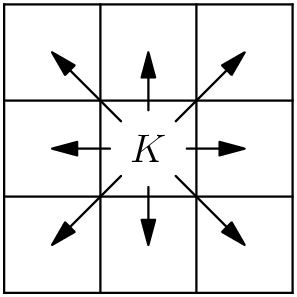
\includegraphics[height=0.3\textheight]{chessking.png}
        \end{figure}
        (A) 20 (B) 24 (C) 27 (D) 28 (E) 32
    
\end{frame}
\begin{frame}{A Typical Problem}
    \begin{theo}[Sticks and Stones]
        The number of ways of placing $n$ indistingushable items into $k$ distinguishable bins is $\binom{n+k-1}{k-1}$.

        If we further assume each bin must contain a positive number of items, the number of ways equals to $\binom{n-1}{k-1}$.
    \end{theo}
    \begin{theo}[Another form of Sticks and Stones]
        Find the number of positive integral solutions and non-negative integral solutions of the equation $x_1+\dots+x_k=n$.
    \end{theo}
\end{frame}
\begin{frame}{Donuts}
    \begin{ques}
        Pat wants to buy four donuts from an ample supply of three types of donuts: glazed, chocolate, and powdered. How many different
        selections are possible?
        帕特想买四个甜甜圈, 卖甜甜圈的商店提供三种选择, 分别为糖霜甜甜圈、巧克力甜甜圈、粉甜甜圈, 这三种甜甜圈供应充足, 请问帕特有几种选择?(注意可以重复购买某一种甜甜圈)
    \end{ques}
        Hint: Consider the equation $x_1+x_2+x_3=4$, where $x_i,i=1,\dots,3$ are all non-negative integers.
\end{frame}
\begin{frame}{Spell AMC8(AMC 8, 2017-15)}
        In the arrangement of letters and numerals below, by how many different paths can one spell AMC8? Beginning at the $A$ in the middle, a path only allows moves from one letter to an adjacent (above, below, left, or right, but not diagonal) letter. One example of such a path is traced in the picture. 
        \begin{figure}
            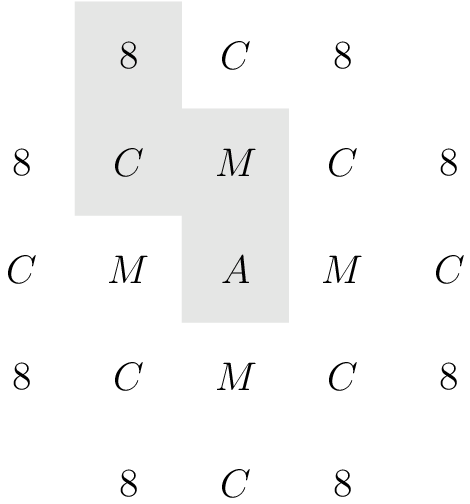
\includegraphics[height=0.3\textheight]{amc8spell.png}
        \end{figure}
        (A) 8 (B) 9 (C) 12 (D) 24 (E) 36
\end{frame}
\begin{frame}{Homework}
    \begin{ques}
        How many positive integers can be represented as a product of two distinct menmbers of the set $\bbrace{1,2,3,4,5,6}$.

        有多少个正整数可以表示为$1,2,3,4,5,6$中两个不同元素的乘积?
    \end{ques}
\end{frame}
\begin{frame}{Homework}
    \begin{ques}
        How many ways can you arrange $7$ people in a row if three of them cannot stand next to each other?

        有多少种方式可以给出七个人$A,B,C,D,E,F,G$的一个排列, 使得$A,B,C$这三个人必须相邻.
    \end{ques}
    \begin{ques}
        (*)Find the number of solutions of the following equation
        \begin{equation*}
            x_1+x_2+x_3=5, x_1\ge 0, x_2,x_3>0, x_i\in \text{are all integers}
        \end{equation*}

        如下方程有多少个解:
        \begin{equation*}
            x_1+x_2+x_3=5, x_1\ge 0, x_2,x_3>0, x_i\,\text{均为整数}
        \end{equation*}
    \end{ques}
\end{frame}
\begin{frame}{Homework}
    \begin{ques}[AMC8, 2020-23]
        Five different awards are to be given to three students. Each student will receive at least one award. In how many different ways can the awards be distributed?

        (A) 120 (B) 150 (C) 180 (D) 210 (E) 240
    \end{ques}
\end{frame}
\end{document}